\section{Ejercicio 5}
Se implementa en Verilog un multiplicador de 2 numeros de un d\'igito en codigo BCD que retorna el resultado como 2 digitos en formato BCD. Incluye adem\'as, un bit de error que ser\'a 1 en caso de que haya un error y 0 en otro caso.

\subsection{Proceso de dise\~no}
En un principio se decidi\'o implementar este sistema a partir de realizar una tabla de verdad y un mapa de Karnaugh. Sin embargo, ese es un punto de vista que si bien parece ser simple, resulta muy engorroso de implementar. Esto se debe a la cantidad de entradas y salidas del sistema, 8 de cada una. Esto requiere resolver 8 mapas, con 8 variables de entrada.
Se opta entonces, por implementarlo emulando la manera en que se resuelven multiplicaciones binarias a mano. Se puede observar en \ref{eq:bin_mult_ex} un ejemplo de lo hablado.
\begin{equation}[H]
    \begin{array}{c}
        \phantom{\times99999}1001\\
        \underline{\times\phantom{9999}0111}\\ %there must be a better way to do this :(((((
        \phantom{\times 999}1001\\
        \phantom{\times 99}1001.\\
        \phantom{\times9}1001..\\        
        \underline{\phantom\times0000...\phantom9}\\
        \phantom\times0111111
    \end{array}
    \label{eq:bin_mult_ex}
\end{equation}


\subsection{Implementac\'on}
En la Figura \ref{fig:circuito_con_FA} se puede observar la implementaci\'on de este proceso con Full-Adders y compuertas AND.

\begin{figure}[H]
    \centering
        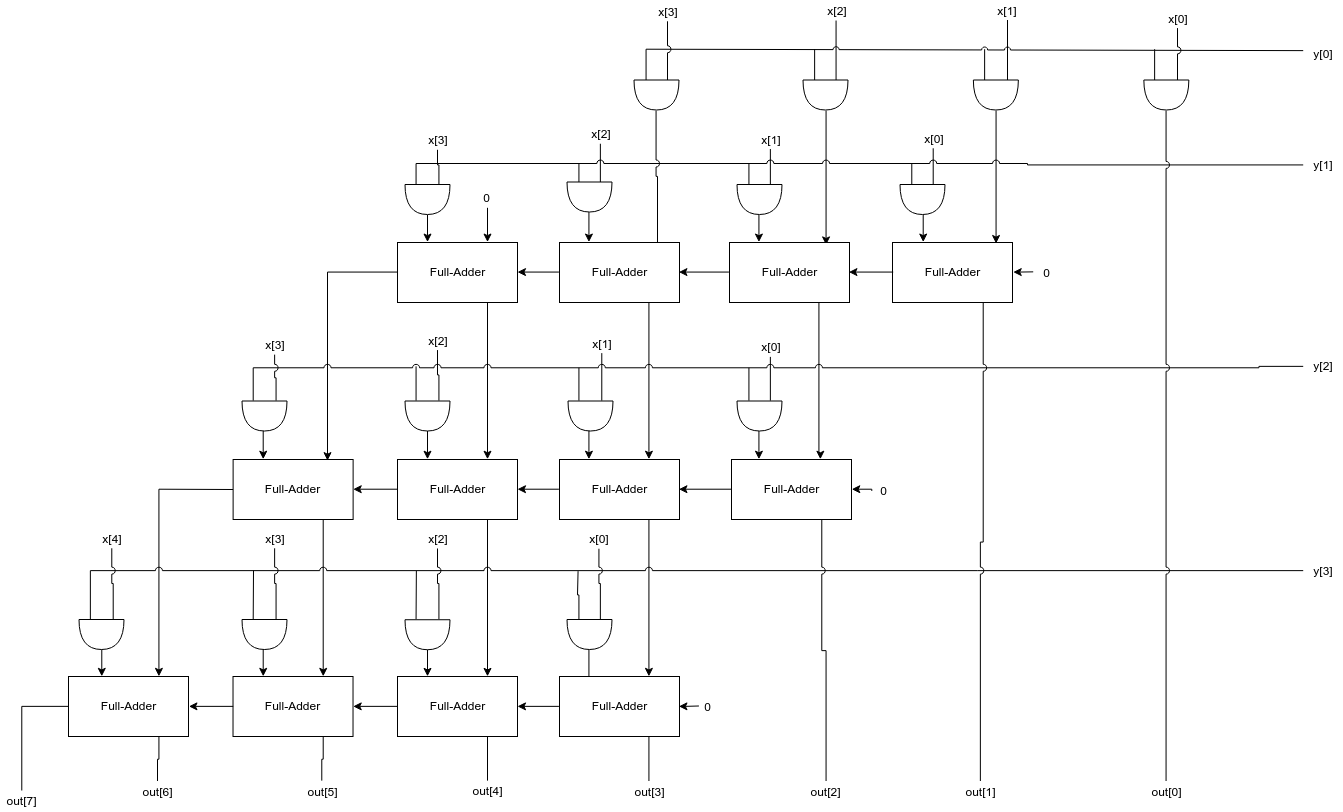
\includegraphics[width=0.9\textwidth]{./EJ_5/circuito_con_FA.png}
        \caption{\label{fig:circuito_con_FA}Circuito l\'ogico que emula el caso descripto.}        
\end{figure}

Este diagrama representa \'unicamente la seccion de la multiplicaci\'on binaria descripta en \ref{eq:bin_mult_ex}, el c\'odigo esta escrito completamente con compuertas l\'ogicas en Verilog.
En cambio, tanto como para validar la informaci\'on recibida como para codificar los resultados binarios en formato BCD se opta por usar bloques \textit{behavioral}.
Se adjunta junto con este informe, el codigo de Verilog con su correspondiente Makefile y un archivo \textit{run}.

\subsection{Test-bench}
Es posible ejecutar un \textit{Test-bench} para verificar que el m\'odulo funciona correctamente, con algunos ejemplos de las posibles entradas al sistema. 
El mismo puede se ejecutado por medio de los comandos:
\begin{lstlisting}[language=bash]
    user@computer: path/to/EJ_5/folder$ make
    user@computer: path/to/EJ_5/folder$ ./run
\end{lstlisting}